\documentclass[aspectratio=169]{beamer}
\usepackage[T1]{fontenc}
\usepackage[utf8]{inputenc}
\usepackage{tikz}
\usepackage{tabularx}
\usepackage[font=scriptsize]{caption}
\captionsetup[figure]{labelformat=empty}

\usetikzlibrary{tikzmark,shapes,arrows,backgrounds,fit,positioning}
\newcolumntype{C}{>{\centering\arraybackslash}X}
\newcolumntype{R}{>{\raggedleft\arraybackslash}X}

\addtobeamertemplate{navigation symbols}{}
{
	\insertframenumber{}
}

\beamertemplatenavigationsymbolsempty
\setbeamercolor{section in foot}{fg=white, bg=blue}
\setbeamercolor{subsection in foot}{fg=black, bg=white}
\setbeamerfont{footline}{size=\fontsize{6}{6}\selectfont}

\setbeamertemplate{footline}
{
  \leavevmode
  \hbox
  {
    \begin{beamercolorbox}
      [wd=.5\paperwidth,ht=2.5ex,dp=1.125ex,leftskip=.3cm,rightskip=.3cm]{subsection in foot}
    \end{beamercolorbox}
    
    \begin{beamercolorbox}
      [wd=.5\paperwidth,ht=2.5ex,dp=1.125ex,leftskip=.3cm,rightskip=.3cm plus1fil]{subsection in foot}
      \hfill
      \insertframenumber
      %\insertframenumber\,/\,\inserttotalframenumber
    \end{beamercolorbox}
  }
}



\title{UUB Charge and Peak histograms}
\author{
  Mauricio Su\'arez Dur\'an and Ioana~C.~Mari\c{s}
}
\institute{IIHE-ULB}

\titlegraphic{
  \begin{figure}[h]
    \centering
   %
\includegraphics[width=5cm]{ulbLogo2.png}
    \hspace*{8.cm}
    
\includegraphics[width=5.5cm]{iihe.jpeg}
  \end{figure}
}

\begin{document}
\begin{frame}
  \titlepage
\end{frame}


\begin{frame}
	\frametitle{UUB Charge and Peak histograms}
	\begin{itemize}
		\item Station studied: 863 1222 1219 1211 1740 1743 1221 1223 1217 1747 1741 1745 1818 1851 1729 1735 1746 1819 1791
		\item Data from CDAS.
		\item {\underline {Software CDAS, pre-production version.}}
	\end{itemize}
	\centering
	\includegraphics[width=.45\textwidth]{mapStations.pdf}
\end{frame}

% ========================
% *** First Bin counts ***

%\begin{frame}
%  \frametitle{UUB and UB counts in the first bin in Raw Peak Histogram}
%	Raw UUB Peak Histogram
%	\begin{figure}
%		\centering
%		\begin{tabularx}{\textwidth}{CC}
%			\begin{tabular}{l}
%				\includegraphics[width=.5\textwidth]{../plots/uubRawPeakPMT1St863.pdf}
%			\end{tabular}
%			&
%			\begin{tabular}{l}
%				\includegraphics[width=.5\textwidth]{../plots/uubRawPeakZoomPMT1St863.pdf}
%			\end{tabular}
%			\\
%			& Not zero counts in the first bin
%		\end{tabularx}
%	\end{figure}
%\end{frame}

\begin{frame}
  \frametitle{UUB Raw Peak histograms: noise at first bin in? }
  {\bf IoSdHisto::Peak[pmtId][0]}
	\begin{figure}
		\centering
    \includegraphics[width=.4\textwidth]{../plots/uubRawPeakPMT1St863.pdf}
		\begin{tabularx}{\textwidth}{CC}
			\begin{tabular}{l}
				%\includegraphics[width=.44\textwidth]{../plots/uubAllAveFrstBinPMTsBars.png}
				\includegraphics[width=.44\textwidth]{../plots/uubAllAveFrstBinPMTs.png}
			\end{tabular}
			&
			\begin{tabular}{l}
        %\includegraphics[width=.44\textwidth]{../plots/ubAllAveFrstBinPMTsBarsFull.png}
				\includegraphics[width=.44\textwidth]{../plots/ubAllAveFrstBinPMTs.png}
			\end{tabular} 
		\end{tabularx}
	\end{figure}
\end{frame}

\begin{frame}
	\frametitle{From UUB raw Peak histogram to correct format}
	{\bf Applying IoSdStation::HPeak method}
	\begin{figure}
		\centering
		\begin{tabularx}{\textwidth}{CC}
      \multicolumn{2}{l}{xp[j] = j*mult + {\bf offset};
      xp[100 + j] = 100 * mult + bigbins * j * mult + {\bf offset}} 
			\\ 
      \begin{tabular}{l}
				\includegraphics[width=.45\textwidth]{../plots/uubPeakPMT1St863.pdf}
			\end{tabular}
      &
      \begin{tabular}{l}
        \includegraphics[width=.38\textwidth]{../plots/uubAllAveOffsetPMTs.png}
        \\
        \includegraphics[width=.38\textwidth]{../plots/ubAllAveOffsetPMTs.png}
      \end{tabular}
		\end{tabularx}
	\end{figure}
\end{frame}

% =======================
% *** For Peak Offset ***

%\begin{frame}
%	{\bf IoSdHisto::Peak[pmtId][0]}
%	\begin{figure}
%		\centering
%		\begin{tabularx}{\textwidth}{CC}
%			\begin{tabular}{l}
%				\includegraphics[width=.48\textwidth]{../plots/uubAllAveOffsetPMTs.png}
%			\end{tabular}
%      &
%      \begin{tabular}{r}
%				\includegraphics[width=.48\textwidth]{../plots/ubAllAveOffsetPMTs.png}
%			\end{tabular}
%		\end{tabularx}
%	\end{figure}
%\end{frame}


% ====================
% *** For Baseline ***

\begin{frame}
	\frametitle{Checking UUB Baseline: IoSdStation::HBase[pmt] and Calib.Base[pmt]}
	\begin{figure}
		\centering
		\begin{tabularx}{\textwidth}{CC}
			\includegraphics[width=.4\textwidth]{../plots/uubAllAveHbasePMTs.png}
			&
      \includegraphics[width=.4\textwidth]{../plots/uubAllAveCalibPMTs.png}
			\\
			\includegraphics[width=.4\textwidth]{../plots/ubAllAveHbasePMTs.png}
			&
			\includegraphics[width=.4\textwidth]{../plots/ubAllAveCalibPMTs.png}
		\end{tabularx}
	\end{figure}
\end{frame}

% ===============================
% *** Correction for Baseline ***

\begin{frame}
	\frametitle{UUB Peak histogram correcting baseline for: HBase and Calib.Base}
	\begin{figure}
		\centering
		\begin{tabularx}{\textwidth}{CC}
			\includegraphics[width=.38\textwidth]{../plots/uubPeakCoorHBasePMT1St863.pdf}
			&
			\includegraphics[width=.38\textwidth]{../plots/uubPeakCoorCalibBasePMT1St863.pdf}
			\\
			\includegraphics[width=.38\textwidth]{../plots/uubPeakCoorHBaseZoomPMT1St863.pdf}
			&
			\includegraphics[width=.38\textwidth]{../plots/uubPeakCoorCalibBaseZoomPMT1St863.pdf}
			\\
			\multicolumn{2}{l}{Is the correction using HBase producing negative bins?}
		\end{tabularx}
	\end{figure}
\end{frame}

% *** For first bin center ***


\begin{frame}
  \frametitle{Comparison PMT1: UUB and UB Peak histogram First Bin center}
  Here, First Bin center: GetBinCenter(1).
  \begin{figure}
    \centering
    \begin{tabularx}{\textwidth}{CC}
			\includegraphics[width=.45\textwidth]{../plots/uubAllAveBinCntrHbasePMTs.png}
			&
			\includegraphics[width=.45\textwidth]{../plots/uubAllAveBinCntrCalibPMTs.png}
      \\
			\includegraphics[width=.45\textwidth]{../plots/ubAllAveBinCntrHbasePMTs.png}
			&
			\includegraphics[width=.45\textwidth]{../plots/ubAllAveBinCntrCalibPMTs.png}
		\end{tabularx}
	\end{figure}
\end{frame}



% ===========================
% *** Applying for Charge ***

%\begin{frame}
%	\frametitle{Applying the previous steps to UUB Charge histograms}
%	{\bf Raw UUB Charge histogram}
%	\begin{figure}
%		\begin{tabularx}{\textwidth}{C}
%			\includegraphics[width=.7\textwidth]{../plots/uubRawChargePMT1St863.pdf}
%		\end{tabularx}
%	\end{figure}
%\end{frame}


\begin{frame}
	\frametitle{Applying the previous steps to UUB Charge histograms}
	{IoSdStation::HCharge}
	\begin{figure}
		\centering
		\begin{tabularx}{\textwidth}{CC}
      \multicolumn{2}{l}{xc[j] = mult*j + {\bf offset}; xc[400+j] = 400*mult + bigbins*mult*j + {\bf offset} }
			\\
			\begin{tabular}{l}
				\includegraphics[width=.38\textwidth]{../plots/uubChargePMT1St863.pdf}
			\end{tabular}
      &
      \begin{tabular}{l}
        \includegraphics[width=.4\textwidth]{../plots/uubAllAveOffsetChPMTs.png}
      \end{tabular}
      \\
      \begin{tabular}{l}
        \includegraphics[width=.4\textwidth]{../plots/uubAllAveOffsetChPMT3s.png}
      \end{tabular}
      &
      \begin{tabular}{l}
        \includegraphics[width=.4\textwidth]{../plots/ubAllAveOffsetChPMTs.png}
      \end{tabular}
		\end{tabularx}
	\end{figure}
\end{frame}

% *** For Offset *** 

%\begin{frame}
%	\frametitle{Comparison all stations: UUB and UB Offset for Charge histograms}
%  \centering
%  \includegraphics[width=.55\textwidth]{../plots/uubAllAveOffsetChPMT3s.png}
%\end{frame}

% ===============
% *** For A/P ***

%\begin{frame}
%  \frametitle{A/P Calculation}
%  {\bf For UB}
%  \begin{figure}
%    \centering
%    \begin{tabularx}{\textwidth}{CC}
%      \includegraphics[width=.4\textwidth]{../plots/ubChargeOffsetBlPMT1.pdf}
%      &
%      \includegraphics[width=.4\textwidth]{../plots/ubChargeOffsetNoBlPMT1.pdf}
%      \\
%      \begin{tabular}{l}
%        \includegraphics[width=.4\textwidth]{../plots/ubChargeNoOffsetPMT1.pdf}
%      \end{tabular}
%      &
%      \begin{tabular}{l}
%        AoP:\\
%        * For Offset - Baseline: 3.1\\
%        * For Offset: 35.5\\
%        * For No offset: 3.7\\
%        * For Peak and Charge No offset: 1.45
%      \end{tabular}
%    \end{tabularx}
%  \end{figure}
%\end{frame}
%
%\begin{frame}
%  \frametitle{A/P Calculation}
%  {\bf For UUB}
%  \begin{figure}
%    \centering
%    \begin{tabularx}{\textwidth}{CC}
%      \includegraphics[width=.4\textwidth]{../plots/uubChargeOffsetBlPMT1.pdf}
%      &
%      \includegraphics[width=.4\textwidth]{../plots/uubChargeOffsetNoBlPMT1.pdf}
%      \\
%      \begin{tabular}{l}
%        \includegraphics[width=.4\textwidth]{../plots/uubChargeNoOffsetPMT1.pdf}
%      \end{tabular}
%      &
%      \begin{tabular}{l}
%        AoP:\\
%        * For Offset - Baseline: NaN\\
%        * For Offset: 8.4\\
%        * For No offset: 8.4\\
%        * For Peak and Charge No offset: 7.9
%      \end{tabular}
%    \end{tabularx}
%  \end{figure}
%\end{frame}

\begin{frame}
  \frametitle{A/P}
  \begin{figure}
    \centering
    \begin{tabularx}{\textwidth}{CC}
      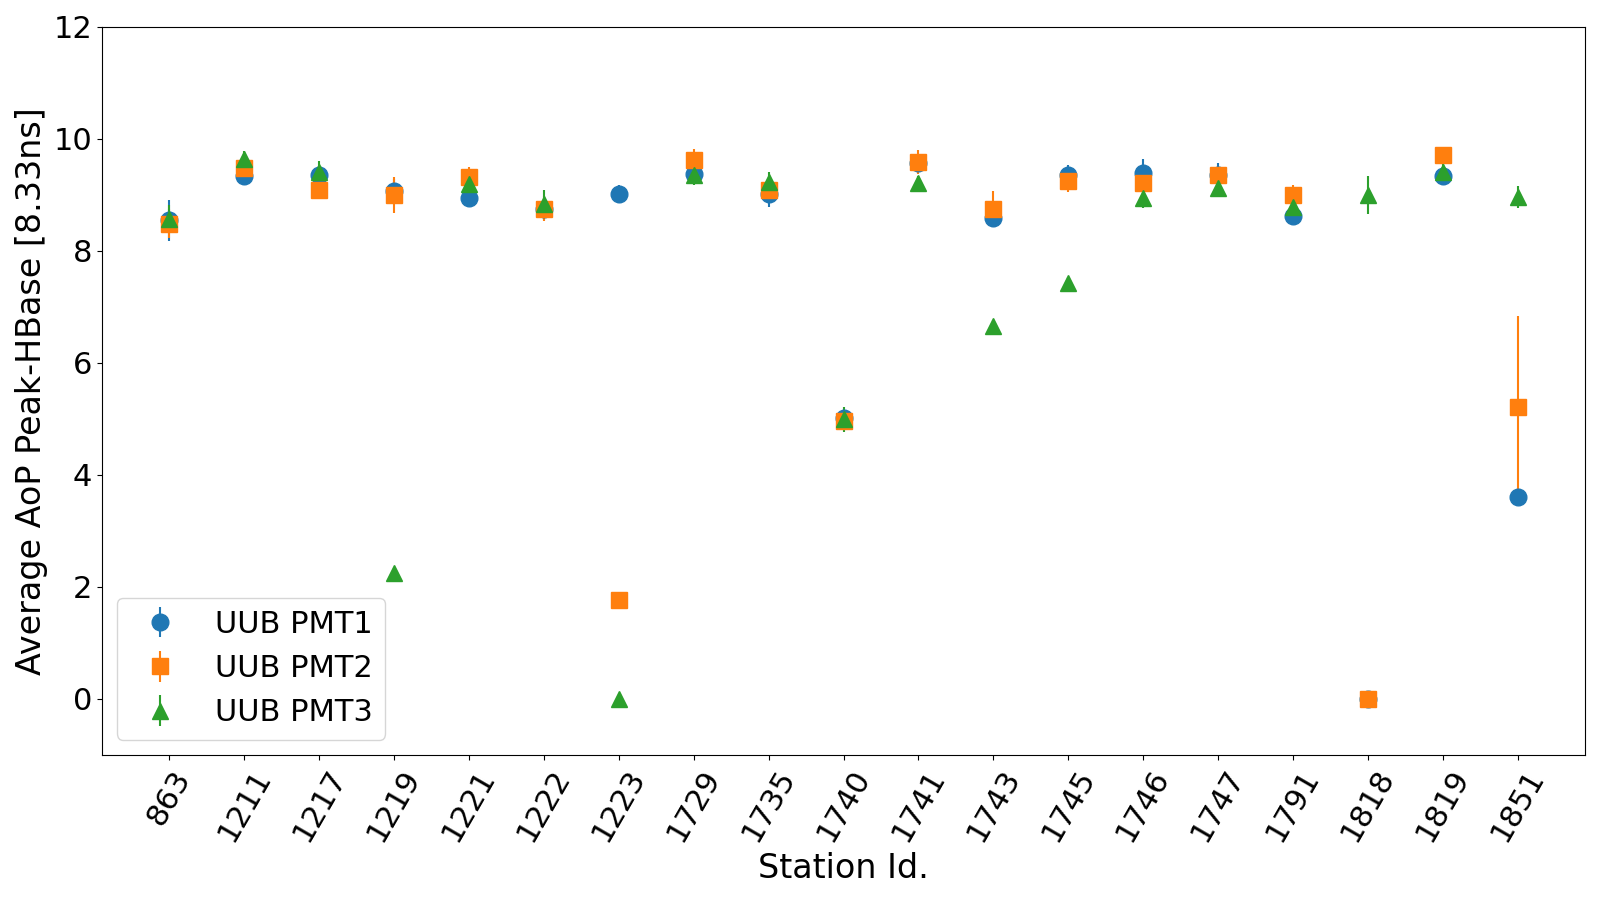
\includegraphics[width=.45\textwidth]{../plots/uubAoPHbasePMTs.png}
      &
      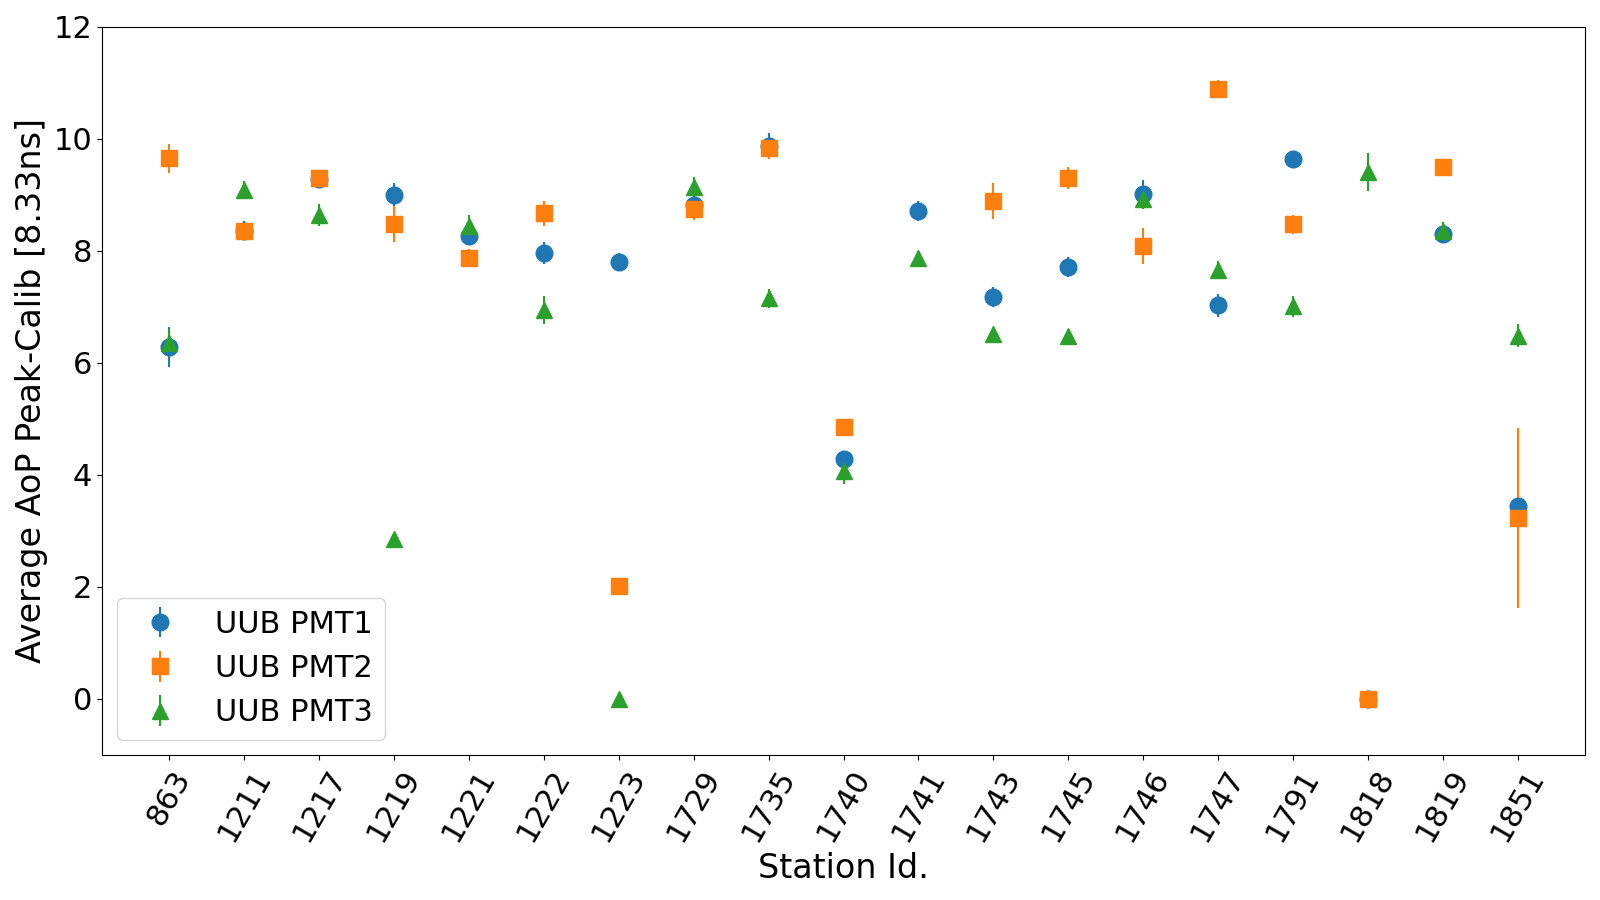
\includegraphics[width=.45\textwidth]{../plots/uubAoPCalibPMTs.png}
      \\
      \includegraphics[width=.45\textwidth]{../plots/ubAoPHbasePMTs.png}
      &
      \includegraphics[width=.45\textwidth]{../plots/ubAoPCalibPMTs.png}
    \end{tabularx}
  \end{figure}
  \centering
  
\end{frame}


\begin{frame}
  \frametitle{A/P Relative difference for Peak corrections}
  \begin{figure}
    PMTs with AoP lower than $4$\,ns for UUB and $2$\,ns for UB are not considered here.
    \centering
    \begin{tabularx}{\textwidth}{CC}
      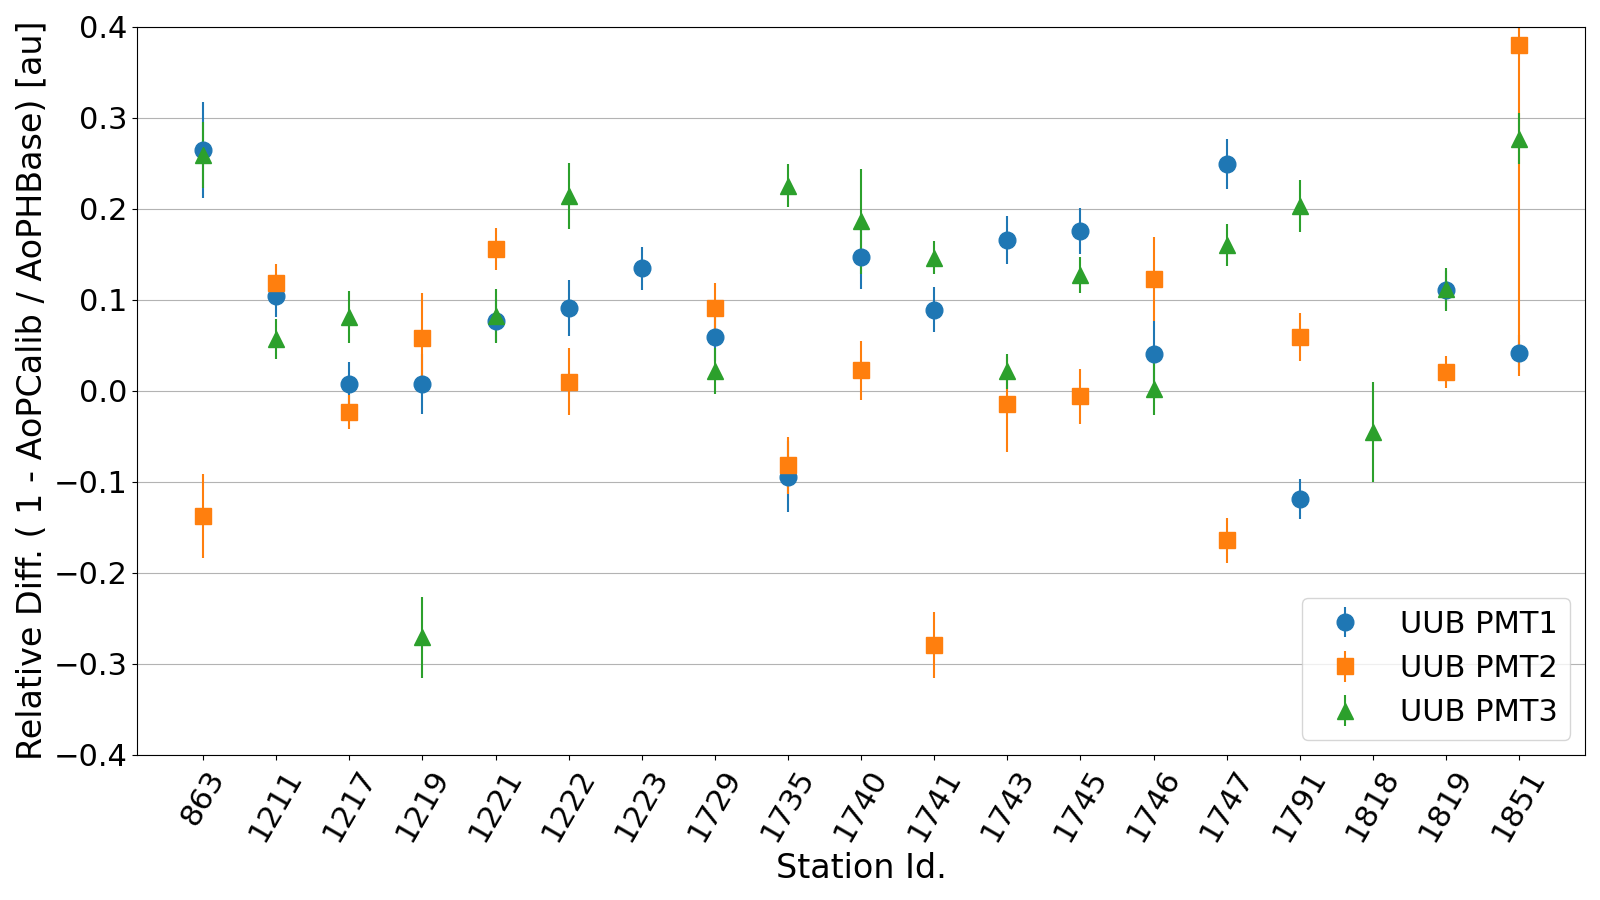
\includegraphics[width=.43\textwidth]{../plots/uubAoPDiffCaHbPMTs.png}
      &
      \includegraphics[width=.43\textwidth]{../plots/ubAoPDiffCaHbPMTs.png}
      \\
      \includegraphics[width=.43\textwidth]{../plots/aopHbaseUubUbPMTs.png}
      &
      \includegraphics[width=.43\textwidth]{../plots/aoCalibUubUbPMTs.png}
    \end{tabularx}
  \end{figure}
\end{frame}



\begin{frame}
  \frametitle{A/P along time}
  \begin{figure}
    \centering
    \begin{tabularx}{\textwidth}{CC}
      \includegraphics[width=.43\textwidth]{../plots/uububAoPtimeHbPMT1St863.png}
      &
      \includegraphics[width=.43\textwidth]{../plots/uububAoPtimeHbPMT1St1743.png}
      \\
      \includegraphics[width=.43\textwidth]{../plots/uububAoPtimeHbPMT3St1740.png}
      &
      \includegraphics[width=.43\textwidth]{../plots/uububAoPtimeHbPMT2St1219.png}
    \end{tabularx}
  \end{figure}
\end{frame}


%\begin{frame}
%  \frametitle{A/P Calculation all stations}
%  \begin{figure}
%    \centering
%    \begin{tabularx}{\textwidth}{CC}
%      \includegraphics[width=.45\textwidth]{../plots/uubAllAoPavePMT1.png}
%      &
%      \includegraphics[width=.45\textwidth]{../plots/ubAllAoPavePMT1.png}
%      \\
%      \includegraphics[width=.45\textwidth]{../plots/uubAllAoPavePMT2.png}
%      &
%      \includegraphics[width=.45\textwidth]{../plots/ubAllAoPavePMT2.png}
%    \end{tabularx}
%  \end{figure}
%\end{frame}
%
%\begin{frame}
%  \frametitle{A/P Calculation all stations}
%  \begin{figure}
%    \centering
%    \begin{tabularx}{\textwidth}{CC}
%      \includegraphics[width=.45\textwidth]{../plots/uubAllAoPavePMT3.png}
%      &
%      \includegraphics[width=.45\textwidth]{../plots/ubAllAoPavePMT3.png}
%    \end{tabularx}
%  \end{figure}
%\end{frame}


% ==============
% *** BACKUP ***

\begin{frame}
  \frametitle{Backup}
\end{frame}

\begin{frame}
  \frametitle{Station 1818}
  \centering
  \includegraphics[width=1.\textwidth]{../plots/st1818pmt3.png}
\end{frame}

\begin{frame}
  \frametitle{Station 1851}
  \centering
  \includegraphics[width=1.\textwidth]{../plots/st1851pmt1.png}
\end{frame}

\begin{frame}
  \frametitle{Station 1219}
  \centering
  \includegraphics[width=1.\textwidth]{../plots/st1219pmt3.png}
\end{frame}

\begin{frame}
  \frametitle{Station 1219}
  \centering
  \includegraphics[width=1.\textwidth]{../plots/st1740pmt3.png}
\end{frame}


%\begin{frame}
%  \frametitle{Improving fit}
%  \begin{figure}
%    \centering
%    \begin{tabularx}{\textwidth}{CC}
%      \includegraphics[width=.55\textwidth]{../plots/uubSmoothOriginalPk.pdf}
%      &
%      \includegraphics[width=.55\textwidth]{../plots/uubSmoothOriginalCh.pdf}
%    \end{tabularx}
%  \end{figure}
%\end{frame}



%\begin{frame}
%  \frametitle{A/P Relative difference for Peak corrections}
%  \begin{figure}
%    \centering
%    \begin{tabularx}{\textwidth}{CC}
%      \includegraphics[width=.5\textwidth]{../plots/uubXiRteXiHbCaPMTs.png}
%      &
%      \includegraphics[width=.5\textwidth]{../plots/ubXiRteXiHbCaPMTs.png}
%    \end{tabularx}
%  \end{figure}
%\end{frame}



\end{document}
